\documentclass[tikz,border=12pt]{standalone}
\usepackage[T1]{fontenc}
\usepackage{lmodern}
\usetikzlibrary{arrows.meta,shapes.geometric}
\tikzset{
  >={Latex[length=2.2mm]},
  every path/.style={line width=.7pt},
  state/.style={draw,line width=1pt,minimum width=4.2cm,minimum height=1cm,font=\small},
  dec/.style={draw,diamond,aspect=2.6,inner sep=1pt,font=\small},
  cond/.style={draw,rounded corners=.5cm,minimum width=3.4cm,minimum height=1cm,font=\small},
  sname/.style={font=\sffamily\bfseries,anchor=south west,inner sep=1pt},
  code/.style={font=\ttfamily\footnotesize,anchor=south east,inner sep=1pt},
  lab/.style={font=\footnotesize,inner sep=1.5pt},
  dot/.style={circle,fill,inner sep=1.4pt}
}
\begin{document}
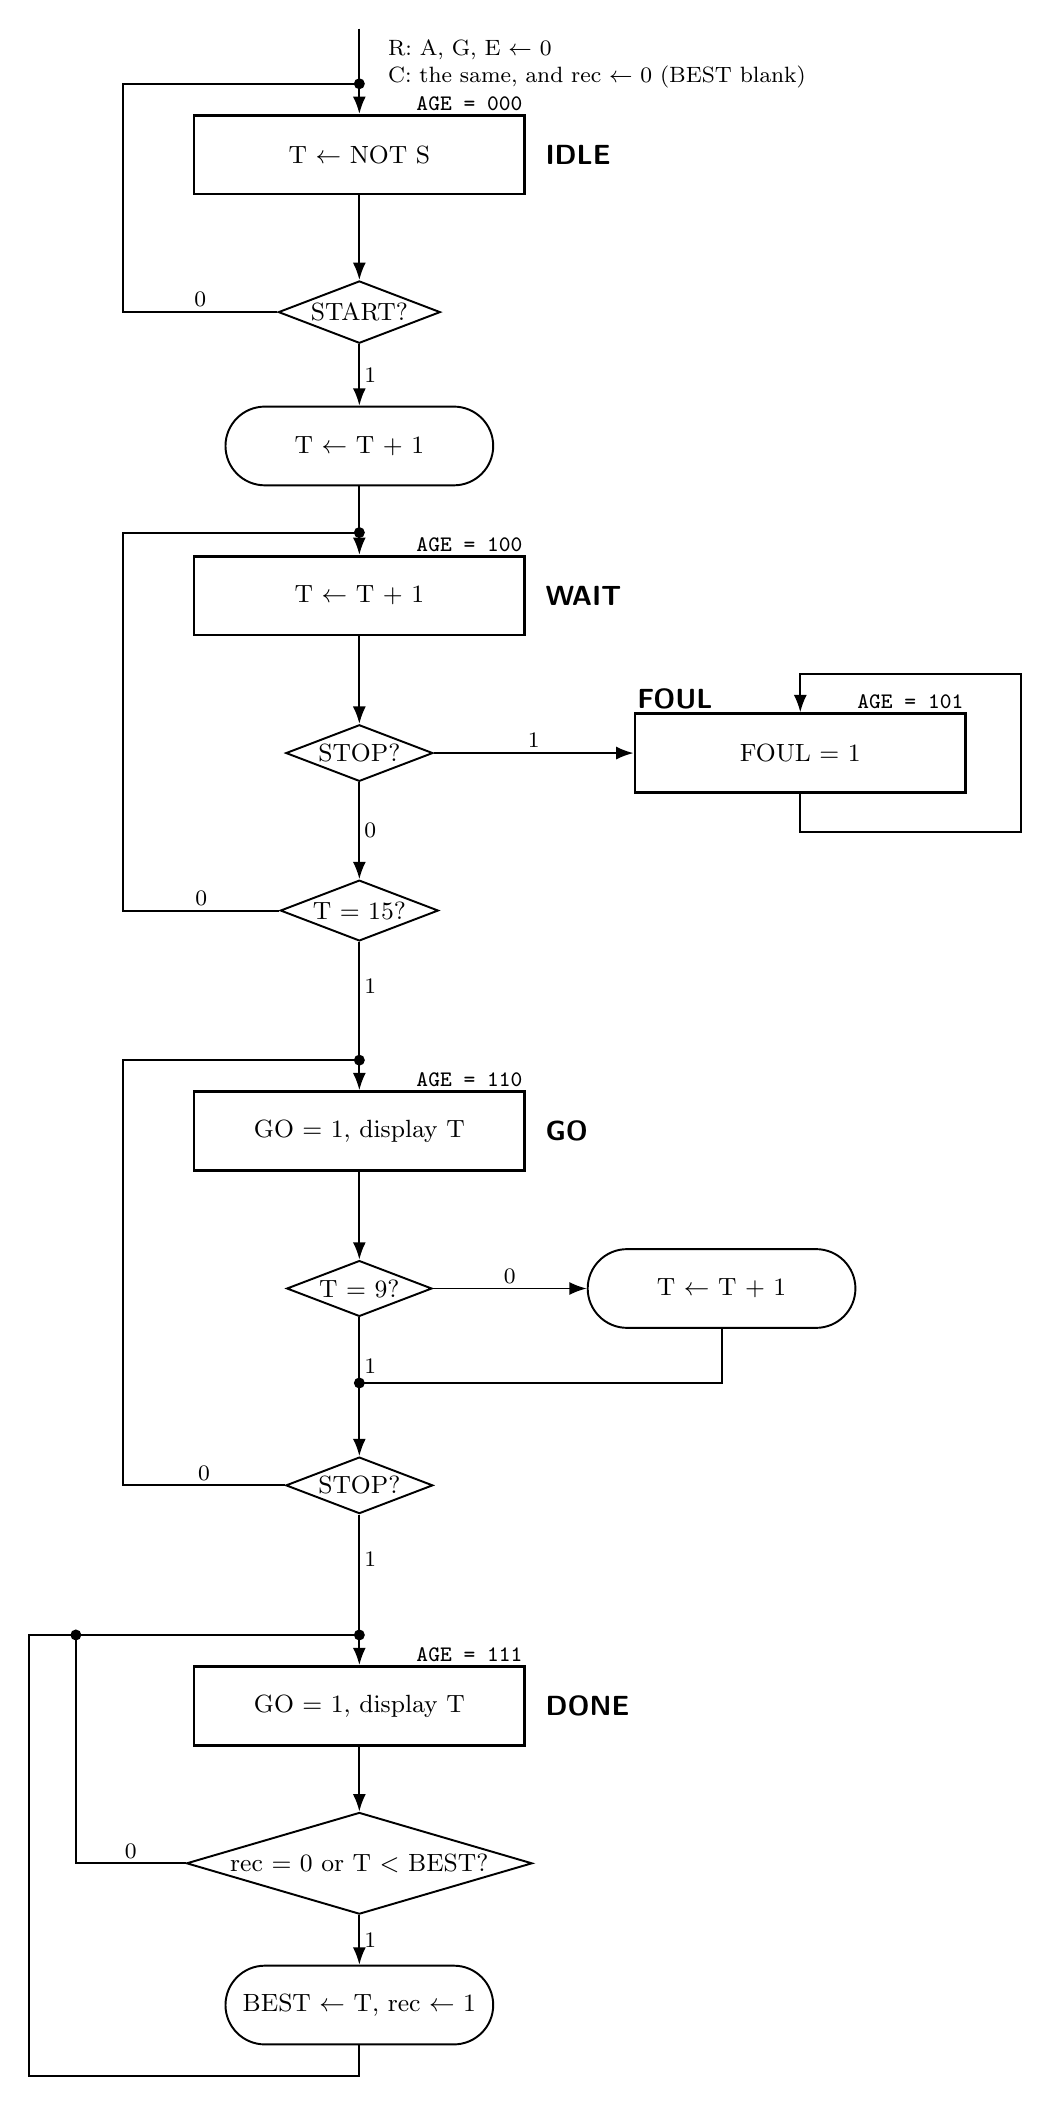
\begin{tikzpicture}
  \node[state] (idle) at (0,0) {T $\leftarrow$ NOT S};
  \node[sname,anchor=west] at ([xshift=2mm]idle.east) {IDLE};
  \node[code] at (idle.north east) {AGE = 000};
  \node[dec] (start) at (0,-2.0) {START?};
  \node[cond] (inc1) at (0,-3.7) {T $\leftarrow$ T + 1};

  \node[state] (wait) at (0,-5.6) {T $\leftarrow$ T + 1};
  \node[sname,anchor=west] at ([xshift=2mm]wait.east) {WAIT};
  \node[code] at (wait.north east) {AGE = 100};
  \node[dec] (stop1) at (0,-7.6) {STOP?};
  \node[dec] (t15) at (0,-9.6) {T = 15?};
  \node[state] (foul) at (5.6,-7.6) {FOUL = 1};
  \node[sname] at (foul.north west) {FOUL};
  \node[code] at (foul.north east) {AGE = 101};

  \node[state] (go) at (0,-12.4) {GO = 1, display T};
  \node[sname,anchor=west] at ([xshift=2mm]go.east) {GO};
  \node[code] at (go.north east) {AGE = 110};
  \node[dec] (t9) at (0,-14.4) {T = 9?};
  \node[cond] (inc2) at (4.6,-14.4) {T $\leftarrow$ T + 1};
  \node[dec] (stop2) at (0,-16.9) {STOP?};

  \node[state] (done) at (0,-19.7) {GO = 1, display T};
  \node[sname,anchor=west] at ([xshift=2mm]done.east) {DONE};
  \node[code] at (done.north east) {AGE = 111};
  \node[dec,aspect=3.4] (better) at (0,-21.7) {rec = 0 or T $<$ BEST?};
  \node[cond] (best) at (0,-23.5) {BEST $\leftarrow$ T, rec $\leftarrow$ 1};

  \draw[->] (0,1.6) -- (idle.north);
  \node[lab,anchor=west,align=left] at (0.3,1.15) {R: A, G, E $\leftarrow$ 0\\C: the same, and rec $\leftarrow$ 0 (BEST blank)};
  \draw[->] (idle) -- (start);
  \draw[->] (start) -- node[lab,right] {1} (inc1);
  \draw[->] (inc1) -- (wait);
  \draw (start.west) -- node[lab,above] {0} (-3.0,-2.0) |- (0,0.9);
  \node[dot] at (0,0.9) {};

  \draw[->] (wait) -- (stop1);
  \draw[->] (stop1.east) -- node[lab,above] {1} (foul.west);
  \draw[->] (stop1) -- node[lab,right] {0} (t15);
  \draw (t15.west) -- node[lab,above] {0} (-3.0,-9.6) |- (0,-4.8);
  \node[dot] at (0,-4.8) {};
  \draw[->] (t15) -- node[lab,right,pos=.3] {1} (go);
  \draw[->] (foul.south) -- (5.6,-8.6) -| (8.4,-6.6) -| (foul.north);

  \draw[->] (go) -- (t9);
  \draw[->] (t9.east) -- node[lab,above] {0} (inc2.west);
  \draw (inc2.south) |- (0,-15.6);
  \node[dot] at (0,-15.6) {};
  \draw[->] (t9) -- node[lab,right,pos=.35] {1} (stop2);
  \draw (stop2.west) -- node[lab,above] {0} (-3.0,-16.9) |- (0,-11.5);
  \node[dot] at (0,-11.5) {};
  \draw[->] (stop2) -- node[lab,right,pos=.3] {1} (done);

  \draw[->] (done) -- (better);
  \draw[->] (better) -- node[lab,right] {1} (best);
  \draw (better.west) -- node[lab,above] {0} (-3.6,-21.7) |- (0,-18.8);
  \draw (best.south) -- (0,-24.4) -| (-4.2,-18.8) -- (-3.6,-18.8);
  \node[dot] at (0,-18.8) {};
  \node[dot] at (-3.6,-18.8) {};
\end{tikzpicture}
\end{document}
